\chapter{Extragalactic extreme-mass-ratio bursts\label{ch:extragal}}

It is well established that space is big \citep[chapter 8]{Adams1979}. The Milky Way, our own island universe, is but one of a multitude of galaxies. Each one of these may have an MBH nestled at its core \citep{Lynden-Bell1971, Soltan1982}. We have considered measuring the properties of the Galaxy's MBH using EMRBs and found that bursts can be informative if the periapsis is small enough. In this chapter, we extend this work to other nearby galaxies. If extragalactic EMRBs are detectable, they may be useful for constraining the properties of those galaxies' MBHs.

We use the NK waveforms from \chapref{waveforms} and the data analysis techniques from \chapref{param}. In \secref{extragal-SNR} we discuss the detectability of EMRBs from extragalactic sources. We show that bursts from other galaxies could be detected with LISA or eLISA. Following this, in \secref{extragal-Res}, we present examples of the constraints we could place using EMRBs. We conclude in \secref{extragal-End} with a discussion of our findings.

\section{Detectability of extragalactic bursts}\label{sec:extragal-SNR}

Whether or not a burst is detectable is determined by its SNR. This is calculated using \eqnref{SNR}. We assume a detection threshold of $\rho = 10$ as in \secref{Gal-SNR}. The SNR of an EMRB depends upon many parameters; for a given MBH, the most important is the periapse radius $r\sub{p}$. There is a good correlation between $\rho$ and $r\sub{p}$. Other parameters specifying the inclination of the orbit, the orientation of the system with respect to the detector, or the MBH spin only produce scatter about this trend. The form of the $\rho$--$r\sub{p}$ relation depends upon the noise curve.

We parametrize the detectability in terms of a characteristic frequency $f_\ast$. The speed at periapse scales like $v \sim \sqrt{GM/r\sub{p}}$; the characteristic time taken for the position to change is then $T \sim r\sub{p}/v$, and so we define the characteristic frequency as
\begin{equation}
f_\ast = \sqrt{\frac{GM_\bullet}{r\sub{p}^3}}.
\end{equation}
This allows comparison between different systems where the same periapse does not correspond to the same frequency and thus the same point of the noise curve.

We also expect the SNR to scale with other quantities. We define a characteristic strain amplitude for a burst $h_0$; we expect $\rho \propto h_0$, where the proportionality will be set by a frequency-dependent function that includes the effect of the noise curve. Assuming that the strain is dominated by the quadrupole contribution (\citealt[section 36.10]{Misner1973}; \citealt[section 17.9]{Hobson2006}) we expect
\begin{equation}
h_0 \sim \frac{G}{c^6}\frac{\mu}{R}\frac{\dd^2}{\dd t^2}\left(r^2\right),
\end{equation}
where $\mu$ is the CO mass, $R$ is the distance to the MBH, $t$ is time and $r$ is a proxy for the position of the orbiting object. The characteristic rate of change is set by $f_\ast$ and the characteristic length-scale is set by $r\sub{p}$. Hence
\begin{align}
h_0 \sim {} & \frac{G}{c^6}\frac{\mu}{R}f_\ast^2 r\sub{p}^2 \\
 \sim {} & \frac{G^{5/2}}{c^6}\frac{\mu}{R}f_\ast^{-2/3}M_\bullet^{2/3}.
\end{align}
Using this, we can factor out the most important dependences to give a scaled SNR defined by
\begin{equation}
\rho_\ast = \left(\frac{\mu}{M_\odot}\right)^{-1}\left(\frac{R}{\mathrm{Mpc}}\right)\left(\frac{M_\bullet}{10^6 M_\odot}\right)^{-2/3}\rho.
\label{eq:SNR-scaling}
\end{equation}

Space-based detectors are most sensitive to extreme-mass-ratio signals originating from systems containing MBHs with masses $\sim10^6 M_\odot$. Higher mass objects produce signals at too low frequencies. We considered several nearby MBHs that were likely candidates for detectable burst signals. Details are given in \tabref{MBHs}.
\begin{table}
%\begin{minipage}{\columnwidth}
 \centering
  \begin{tabular}{P{0.22\textwidth} c  D{.}{.}{2.5} P{0.4\textwidth}}
  \toprule
   Galaxy & \multicolumn{1}{c}{$M_\bullet/10^6 M_\odot$} & \multicolumn{1}{c}{$R/\mathrm{Mpc}$} & References \\
 \midrule
 Milky Way (Sgr A*) & $4.31 \pm 0.36$ & 0.00833 & \citet{Gillessen2009} \\
 Andromeda (M31, NGC 224) & $140^{+90}_{-30}$ & 0.770 & \citet{Bender2005,Karachentsev2004} \\
 M32 (NGC 221) & $2.5 \pm 0.5$ & 0.770 & \citet{Verolme2002,Karachentsev2004} \\
 Circinus & $1.1 \pm 0.2$ & 2.82 & \citet{Graham2008,Greenhill2003,Karachentsev2007} \\
 NGC 4945 & $1.4^{+0.7}_{-0.5}$ & 3.82 & \citet{Greenhill1997,Ferrarese2005,Karachentsev2007} \\
 Sculptor (NGC 253) & $10^{+10}_{-5}$ & 3.5 & \citet{Graham2011,Rodriguez-Rico2006,Rekola2005} \\
 NGC 4395 & $0.36 \pm 0.11$ & 4.0 & \citet{Peterson2005,Thim2004} \\
 M96 (NGC 3368) & $7.3 \pm 1.5$ & 10.1 & \citet{Graham2011,Nowak2010,Tonry2001} \\
 NGC 3489 & $5.8 \pm 0.8$ & 11.7 & \citet{Graham2011,Nowak2010,Tonry2001} \\
\bottomrule
\end{tabular}
\caption{Sample of nearby MBHs that are candidates for producing detectable EMRBs.\label{tab:MBHs}}
%\end{minipage}
\end{table}
For each, we calculated SNRs at $\sim 10^4$ different periapse distances, uniformly distributed in log space between the innermost orbit and $100 r\sub{g}$ following the procedure in \secref{wave-ex}: for each periapse, five SNRs were calculated using different sets of ancillary parameters specifying the spin magnitude and orientation of the MBH, the orbital inclination and phase, and the position of the detector.

The scaled SNRs are plotted in \figref{scaled-SNR}. The plotted points are the average values of $\ln \rho_\ast$ calculated for each periapse distance.
\begin{figure}
\begin{center}
 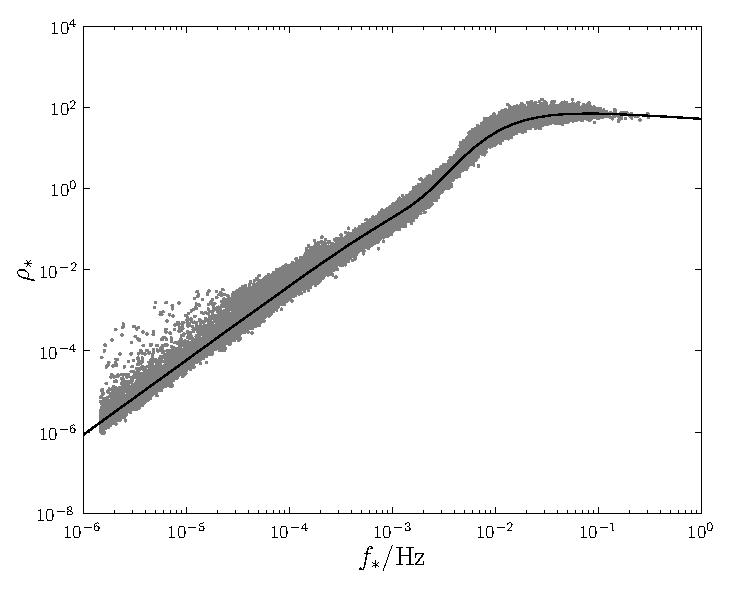
\includegraphics[width=0.6\textwidth]{./images/Fig_SNR_scaled_fit}
 \caption{Scaled SNR for EMRBs as a function of characteristic frequency. The fitted curve from \eqnref{scaled-SNR} is indicated by the line.\label{fig:scaled-SNR}}
   \end{center}
\end{figure}
The curve shows that EMRB SNR does scale as expected, and $\rho_\ast$ can be described as a one-parameter curve. There remains some scatter about this: the larger scatter at low frequencies is a consequence of numerical noise from dealing with very low SNRs from Andromeda; removing the averaging over ancillary parameters increases the scatter to be typically about an order of magnitude in total. However, the fit is good enough for rough calculations.

We approximate the trend with a parametrized curve
\begin{equation}
\rho_\ast = \alpha_1 \left(\frac{f_\ast}{\mathrm{Hz}}\right)^{\beta_1} \left[1 + \left(\alpha_2 \frac{f_\ast}{\mathrm{Hz}}\right)^{\beta_2}\right]\left[1 + \left(\alpha_3 \frac{f_\ast}{\mathrm{Hz}}\right)^{\beta_3}\right]^{-\beta_4}.
\label{eq:scaled-SNR}
\end{equation}
To fit this, we treat the problem as if it were a likelihood maximisation, with each averaged point having a Gaussian likelihood with standard deviation defined from the scatter because of the variation in the ancillary parameters. The optimised values for LISA are
\begin{equation}
\begin{split}
\alpha_1 \simeq 8.93 \times 10^4; \quad \alpha_2 \simeq 4.68 \times 10^2; \quad \alpha_3 \simeq 1.84 \times 10^2;\\
\beta_1 \simeq 1.84; \quad\beta_2 \simeq 3.23; \quad \beta_3 \simeq 1.27; \quad \beta_4 \simeq 4.13.
\end{split}
\end{equation}

Using our fitted trends, it is possible to invert \eqnref{SNR-scaling} to find the furthest distance that a system contain an MBH of a given mass can produce detectable bursts. In calculating the maximum SNR it is necessary to decide upon a maximum $f_\ast$. This corresponds to the minimum periapse radius which is in turn determined by the MBH spin. For the optimal case with a maximally rotating MBH, the innermost periapsis is $r\sub{p} = r\sub{g}$; for a non-rotating MBH, the innermost periapsis would be $r\sub{p} = 4r\sub{g}$. We shall use both as limits for the maximum SNR.

\Figref{detect} shows the detectability limit for $\mu = 1 M_\odot$ and $\mu = 10 M_\odot$ COs. In addition to the sample of MBHs from \tabref{MBHs} we plot additional nearby MBHs \citep[see][and references therein]{Graham2008,Graham2011,Graham2013}.
\begin{figure}
\begin{center}
 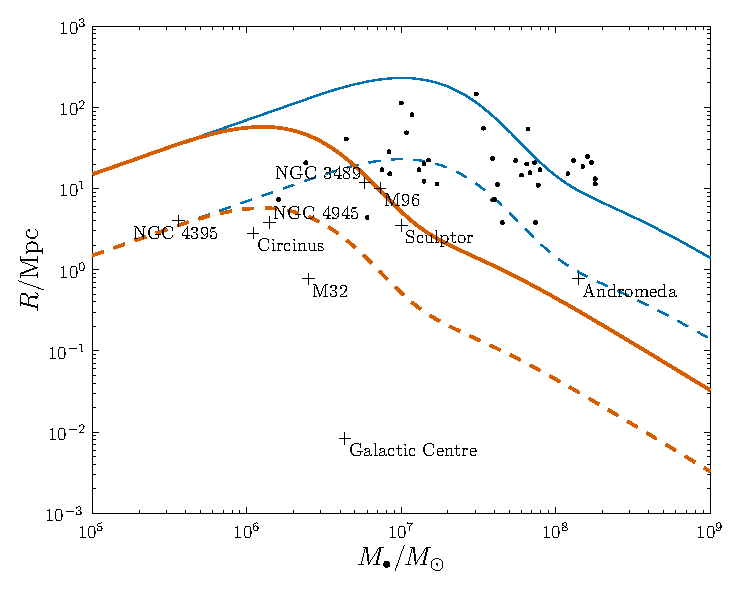
\includegraphics[width=0.6\textwidth]{./images/Fig_M_R_detect_1}
 \caption{Limit of detection using LISA for EMRBs originating from MBHs of mass $M$ and distance $R$ with CO of mass $\mu = 1 M_\odot$ (dashed line) or $\mu = 10 M_\odot$ (solid line). The detection threshold is assumed to be $\rho = 10$. The thicker line is the limit for non-rotating MBHs, the thinner is for maximally rotating MBHs. Sources below the relevant line are potentially detectable. The crosses indicate the selected sample of MBHs used to calibrate the curve and the dots indicate other nearby MBHs with known masses. The trends should not be extrapolated to lower MBH masses.\label{fig:detect}}
   \end{center}
\end{figure}
The more massive COs are detectable to a greater distance, but are also the more likely sources since mass segregation ensures that they are more likely to be on orbits that pass close to the MBH \citep{Bahcall1977, Alexander2009, Preto2010}. Limits using periapsis of $r\sub{g}$ and $4r\sub{g}$ are shown: intermediate spin values would have limits between these two. In any case, these are strict bounds; it is unlikely that we would observe a burst from the optimal orbit. Therefore bursts from MBHs outside the curve are impossible to detect and those inside may be possible, but need not be probable, to detect.

It appears that there are many extragalactic MBHs which could produce observable bursts. From the sample in \tabref{MBHs} all could be detected. Andromeda could only be detected if it has a high spin value. It is therefore less promising than the others. NGC 3489, M96 and Sculptor lie on the boundary of detectability for non-spinning sources with a $10 M_\odot$ CO. They are therefore of marginal interest: we do not necessarily need any special requirement for the spin, but such close orbits would be infrequent. NGC 4395, NGC 4945 and Circinus are around the boundary of detectability for a $1 M_\odot$ CO. Hence, we could potentially see bursts from white dwarfs or neutron stars as well as BHs. M32 is the best extragalactic source, lying safely within the detection limit for $1 M_\odot$ COs. Outside of our sample there are other MBHs with measured masses that are of interest. A great many could potentially be detected using optimal bursts from $10 M_\odot$ COs orbiting a maximally rotating MBH.\footnote{Many galaxies of the Virgo cluster fall in this category. This could potentially make identifying the source galaxy more difficult as the candidates are close together. Since we would have to be fortunate to encounter this problem, we shall not be overly concerned by it.} The most promising MBHs not included in our test sample are found in M64 (NGC 4826), NGC 3076 and M94 (NGC 4736).

We can repeat the analysis for eLISA. The scaled SNRs are shown in \figref{scaled-SNR-eLISA}.
\begin{figure}
\begin{center}
 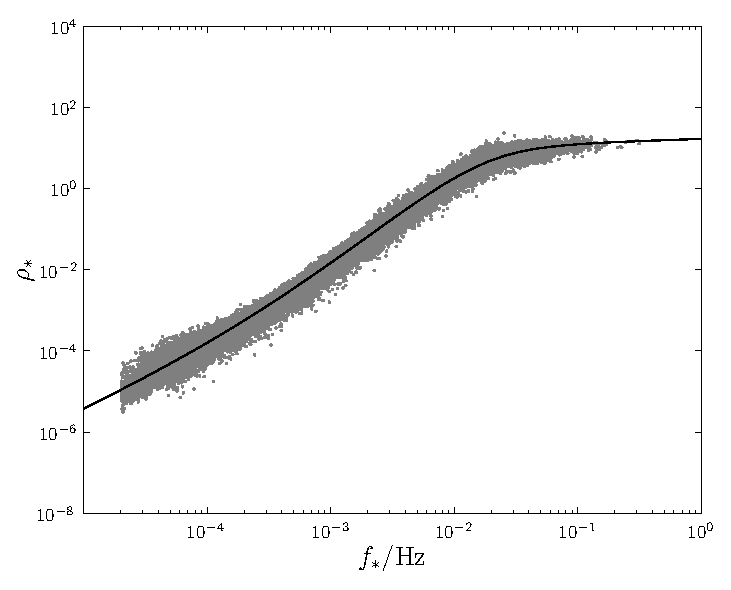
\includegraphics[width=0.6\textwidth]{./images/Fig_SNR_scaled_fit_eLISA}
 \caption{Scaled SNR for EMRBs as a function of characteristic frequency for the eLISA design. The fitted curve from \eqnref{scaled-SNR} is indicated by the line.\label{fig:scaled-SNR-eLISA}}
   \end{center}
\end{figure}
Since Andromeda was only marginally of interest for the classic LISA design, we did not include it this time. This reduces the scatter at low characteristic frequencies.

The curve is fitted with
\begin{equation}
\begin{split}
\alpha_1 \simeq 73.9; \quad \alpha_2 \simeq 4.99 \times 10^3; \quad \alpha_3 \simeq 52.7;\\
\beta_1 \simeq 1.47; \quad\beta_2 \simeq 0.85; \quad \beta_3 \simeq 1.76; \quad \beta_4 \simeq 1.25.
\end{split}
\end{equation}
The fit parameters are markedly different from those for LISA. However, since we are fitting a phenomenological model and the parameters have no physical significance, we are not concerned with this. The parameters yield a good fit to the data, which is all that we are concerned about here.

Using this fit to find the detectability range results in the curves shown in \figref{detect-eLISA}.
\begin{figure}
\begin{center}
 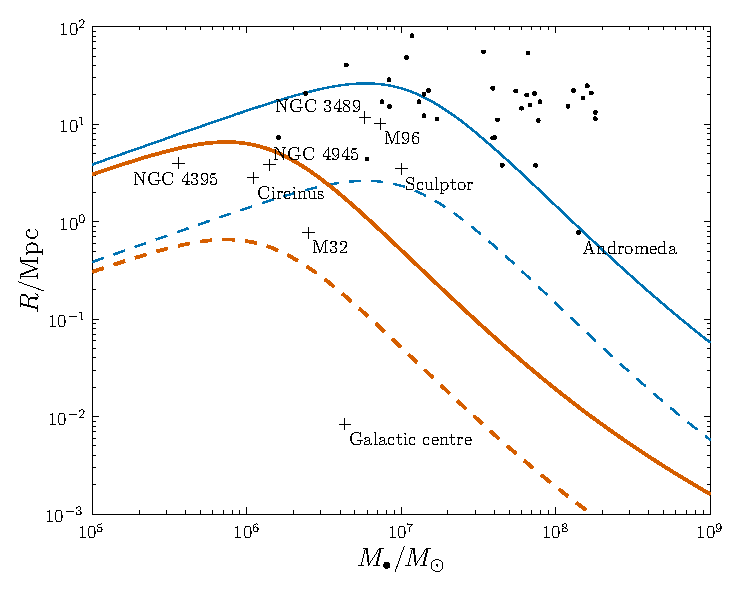
\includegraphics[width=0.6\textwidth]{./images/Fig_M_R_detect_2}
 \caption{Limit of detection using eLISA for EMRBs originating from MBHs of mass $M$ and distance $R$ with CO of mass $\mu = 1 M_\odot$ (dashed line) or $\mu = 10 M_\odot$ (solid line). The detection threshold is assumed to be $\rho = 10$. The thicker line is the limit for non-rotating MBHs, the thinner is for maximally rotating MBHs. Sources below the relevant line are potentially detectable. The crosses indicate the selected sample of MBHs used to calibrate the curve and the dots indicate other nearby MBHs with known masses. The trends should not be extrapolated to lower MBH masses.\label{fig:detect-eLISA}}
   \end{center}
\end{figure}
The maximum distances are reduced compared to the LISA case indicating that detectable bursts would be much rarer. There still remain a number of potential candidate galaxies. From our sample, Andromeda is on the very edge of possibility. NGC 3489, M96 and Sculptor require a high spin, making them unlikely sources. NGC 4395, NGC 4945 and Circinus can be detected without the high spin assuming a $10 M_\odot$ CO. Of the extragalactic sources, only M32 remains detectable with a $1 M_\odot$ CO, and still it requires a non-zero spin.

Using either noise curve we see that EMRBs could potentially be seen from a range of galaxies. The Galaxy's MBH remains securely detectable in either case. M32 is the next best. MBHs with masses $\sim 10^6$--$10^7 M_\odot$ are observable to the greatest distance. We currently know of few MBHs with masses at the lower end of the spectrum ($10^5$--$10^6 M_\odot$) but these would be good potential candidates.

\section{Parameter estimation using extragalactic bursts}\label{sec:extragal-Res}

We are not only interested in discovering if EMRBs are detectable, but also if we can extract information from the signals about their sources. To investigate the potential of extragalactic EMRBs, we considered a sample of bursts from M32, the most promising candidate; NGC N4945, which is near to the optimal mass for LISA (without assuming spin), and NGC 4395, the lightest MBH in our sample. Circinus is similar to NGC 4945, so we expect comparable results: EMRBs from Circinus should be slightly more useful as Circinus is closer.

\subsection{Parameter inference}

In determining parameters from burst waveforms, we have the same inference problem as in \secref{Estimation}. Our parameter set, as previously enumerated in \secref{Mod-param}, consists of:
\begin{enumerate}[leftmargin=*, widest=\:88--88.]
\item[1.] The MBH's mass $M_\bullet$.
\item[2.] The spin parameter $a_\ast$.
\item[3, 4.] The orientation angles for the MBH spin $\Theta\sub{K}$ and $\Phi\sub{K}$.
\item[5.] The source distance $R$ divided by the CO mass $\mu$, which we denote as $\zeta = R/\mu$. This scales the amplitude of the waveform.
\item[6, 7.] The angular momentum of the CO parametrized in terms of total angular momentum $L_\infty$ and inclination $\iota$.
\item[8--10.] The angular phases at periapse, $\phi\sub{p}$  and $\chi\sub{p}$ (which determines $\theta\sub{p}$), and the time of periapse $t\sub{p}$.
\item[11, 12.] The coordinates of the source. Sky position is already determined to high accuracy for each galaxy. Since an EMRB can only give weak constraints on source position we take it as known and do not infer it.
\item[13, 14.] The orbital position of the detector. This should be known and need not be inferred. We assume the same initial position as \citet{Cutler1998}; this does not qualitatively influence results.
\end{enumerate}
We are interested in inferring the first $10$. The most interesting are the MBH's mass and spin, as these give an insight into the evolution of the MBH's host galaxy. We have estimates for many extragalactic MBHs' masses, but these are less accurate than for the Galactic MBH.

We have assumed that sky position is known; to be able to do this in practice we must be able to successfully identify the source galaxy. We shall see that there are only a few potential galaxies that could produce detectable EMRBs. It should therefore not be too computationally expensive to check all the candidate sky positions. If multiple galaxies lie close together on the sky, such that they cannot be distinguished, it could be possible to use constraints on the MBH mass to differentiate them. This would not help with galaxies for which we do not have good MBH mass estimates.

\subsection{Mapping the posterior distribution}

To discover if any parameters can be accurately inferred, we must characterise the shape of the posterior. We do this using the MCMC techniques developed in \secref{MCMC}. The only modification was to lower the target acceptance rate to $\sim0.08$. This appeared to give improved convergence for these less-informative distributions.

As for bursts from the Galactic Centre, posteriors can show strong and complicated parameter degeneracies. The lower SNR compared to Galactic bursts yields wider distributions. As the periapsis increases, the posteriors deteriorate, becoming uninformative. The posteriors recovered from our MCMC show a wide variety of forms. There is a spectrum from well-formed Gaussians through elongated ellipsoids to complete covering of the parameter range. Some example results are shown in \figref{MCMC-a}, \ref{fig:MCMC-b} and \ref{fig:MCMC-c}. These are similar to the plots in \secref{Gal-Results} except that we now plot $\ln(M_\bullet/M_\odot)$ and $\ln(\zeta/\zeta_0)$.

\begin{figure}
\begin{center}
\vspace{0.5\baselineskip}
   \includegraphics[width=0.82\textwidth]{./images/Fig_M32_MCMC_193_triangle_40}
\caption{Marginalised one- and two-dimensional posteriors (on the diagonal and above, respectively). The scales are identical in both types of plots. The dotted line indicates the true value. These distributions are exceptionally cromulent and well converged. Angular momentum is in units of $L_\bullet = GM c^{-1}$ and the scaled distance is in units of $\zeta_0 = 1 M_\odot^{-1}\units{kpc}$. The EMRB is from M32 and has $r\sub{p} \simeq 5.53 r\sub{g}$.\label{fig:MCMC-a}}
\end{center}
\end{figure}
\Figref{MCMC-a} shows the posterior for an EMRB from M32 with $r\sub{p} \simeq 5.53 r\sub{g}$. The distribution is well-defined and near Gaussian, although even in this best case the presence of degeneracies is clear. This example illustrates that it is possible to obtain good results, similar to those from the Galactic Centre, from extragalactic sources. Unfortunately, such tight distributions are not common in our sample.

\begin{figure}
\begin{center}
\vspace{0.5\baselineskip}
   \includegraphics[width=0.82\textwidth]{./images/Fig_N4395_MCMC_120_triangle_40}
\caption{Marginalised one- and two-dimensional posteriors. The conventions are the same as in \figref{MCMC-a}. These distributions begin to show the complicated shapes of degenerate distributions. The EMRB is from NGC 4395 and has $r\sub{p} \simeq 5.92 r\sub{g}$.\label{fig:MCMC-b}}
\end{center}
\end{figure}
\Figref{MCMC-b} shows the posterior for an EMRB from N4395 with $r\sub{p} \simeq 5.92 r\sub{g}$; it illustrates a more usual posterior. Typical posteriors are not Gaussian; the forms vary significantly, such that it is not possible to produce a standard shape. Non-Gaussianity manifests by the distributions broadening, developing curves and becoming banana-like. The degeneracies may evolve such that there are multiple modes.

\begin{figure}
\begin{center}
	\vspace{0.5\baselineskip}
   \includegraphics[width=0.82\textwidth]{./images/Fig_M32_MCMC_159_triangle_40}
\caption{Marginalised one- and two-dimensional posteriors. The conventions are the same as in \figref{MCMC-a}. These are the worst-case scenario distributions that are uninformative. The EMRB is from M32 and has $r\sub{p} \simeq 11.79 r\sub{g}$.}
\label{fig:MCMC-c}
\end{center}
\end{figure}
\Figref{MCMC-c} shows the culmination of the deterioration of the posterior; it is for an EMRB from M32 with $r\sub{p} \simeq 11.79 r\sub{g}$. In this case, the distributions have extended to encompass the entire range for some parameters and so the EMRB is (near) useless. The posteriors show intricate degeneracies in some angular parameters. These are naturally periodic and demonstrate that near identical bursts can be produced through various rotations of the MBH and orbit. Such bursts are not informative and so are not of interest, but we include this example so that there is no illusion of all EMRBs having perfect posteriors.

The general trend is for bursts from orbits with smaller periapses to be narrower and more Gaussian. As the periapse increases, and SNR decreases, the distributions broaden becoming more non-Gaussian. Curving degeneracies and secondary modes develop. Eventually, the distribution broadens to encompass the entire permitted range for the spin and various angular parameters, effectively making these quantities unconstrained.

\subsection{Parameter uncertainties}

Characteristic distribution widths for the (logarithm of the) MBH mass and the spin are shown in \figref{sigmas-M32}, \ref{fig:sigmas-N4945} and \ref{fig:sigmas-N4395} for M32, NGC 4945 and NGC 4395 respectively. Plotted are the standard deviation $\sigma\sub{SD}$ and the half-width of the $p = 0.68$ range calculated from the $k$-d tree $\sigma_{0.68}$. These widths are defined in \secref{k-d} and are equal for a normal distribution. The filled circles are used for runs that appear to have converged. The open circles are for those yet to converge, but which appear to be approaching an equilibrium state; widths should be accurate to within $\sim 10\%$.
\begin{figure}
\begin{center}
\subfigure[Natural logarithm of MBH mass.]{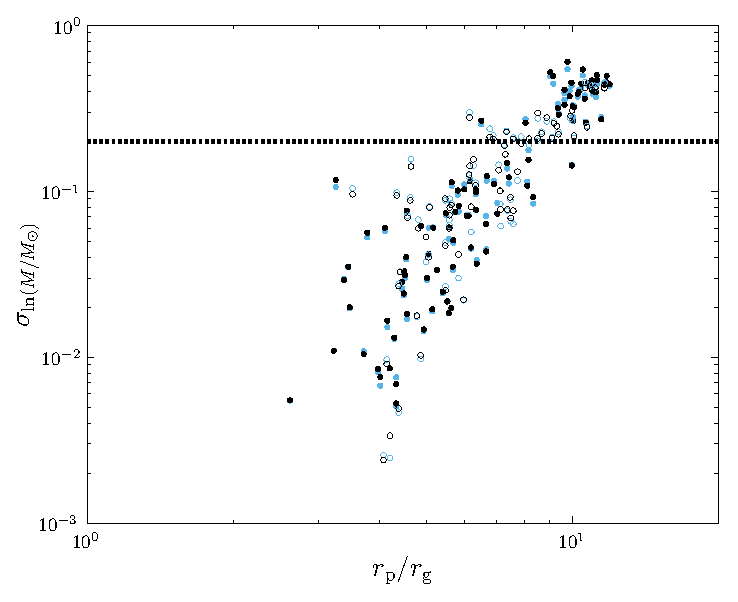
\includegraphics[width=0.475\textwidth]{./images/Fig_M32_MCMC_sigmas_rp_1}} \quad
\subfigure[Dimensionless spin.]{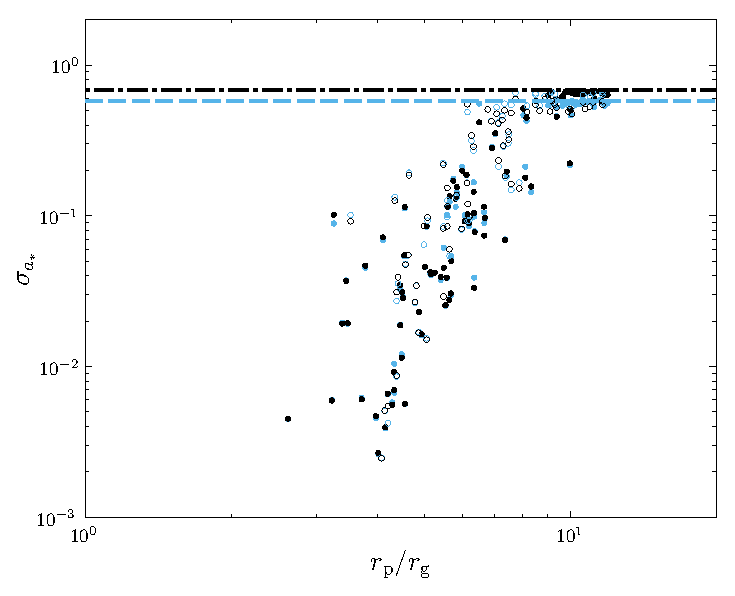
\includegraphics[width=0.475\textwidth]{./images/Fig_M32_MCMC_sigmas_rp_2}} \\
\caption{Distribution widths as functions of periapsis $r\sub{p}$ for M32. The light blue points are used for the standard deviation, the black for the $68$-percentile half-width. The filled circles are converged runs and the open circles for those yet to converge. The dotted line is the current uncertainty for $M_\bullet$. The dashed line is the standard deviation for a uniform $a_\ast$ distribution and the dot--dashed line is the equivalent $68$-percentile half-width.\label{fig:sigmas-M32}}
\end{center}
\end{figure}
\begin{figure}
\begin{center}
\subfigure[Natural logarithm of MBH mass.]{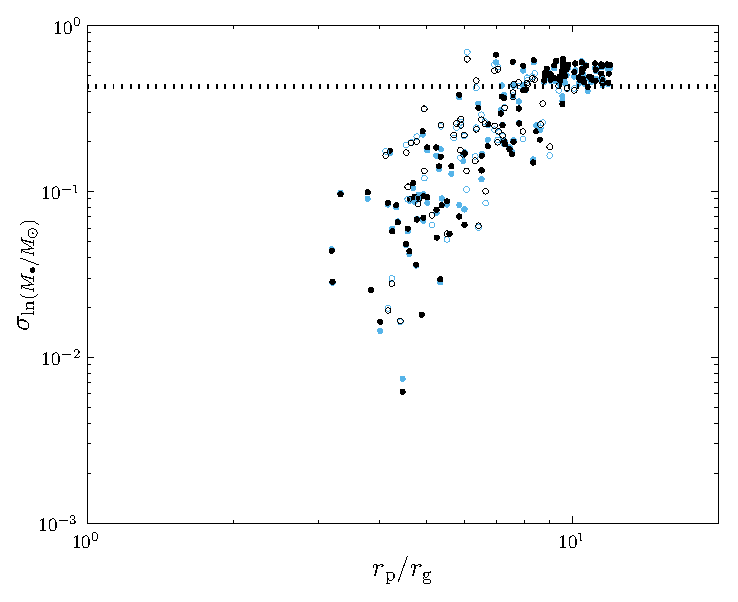
\includegraphics[width=0.475\textwidth]{./images/Fig_N4945_MCMC_sigmas_rp_1}} \quad
\subfigure[Dimensionless spin.]{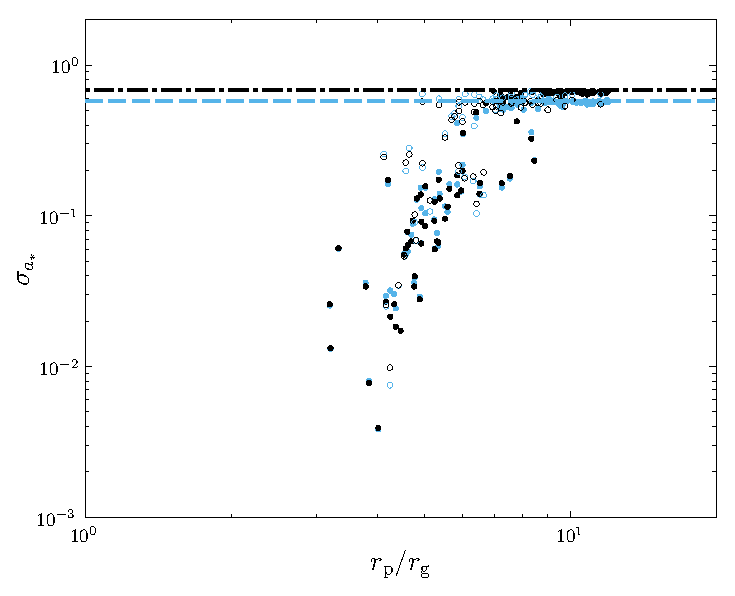
\includegraphics[width=0.475\textwidth]{./images/Fig_N4945_MCMC_sigmas_rp_2}} \\
\caption{Distribution widths as functions of periapsis $r\sub{p}$ for NGC 4945. Conventions are identical to those in \figref{sigmas-M32}.\label{fig:sigmas-N4945}}
\end{center}
\end{figure}
\begin{figure}
\begin{center}
\subfigure[Natural logarithm of MBH mass.]{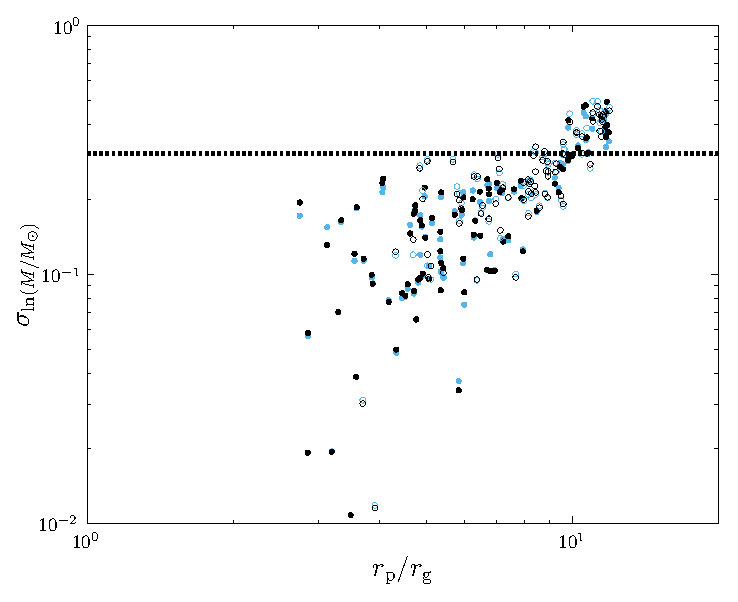
\includegraphics[width=0.475\textwidth]{./images/Fig_N4395_MCMC_sigmas_rp_1}} \quad
\subfigure[Dimensionless spin.]{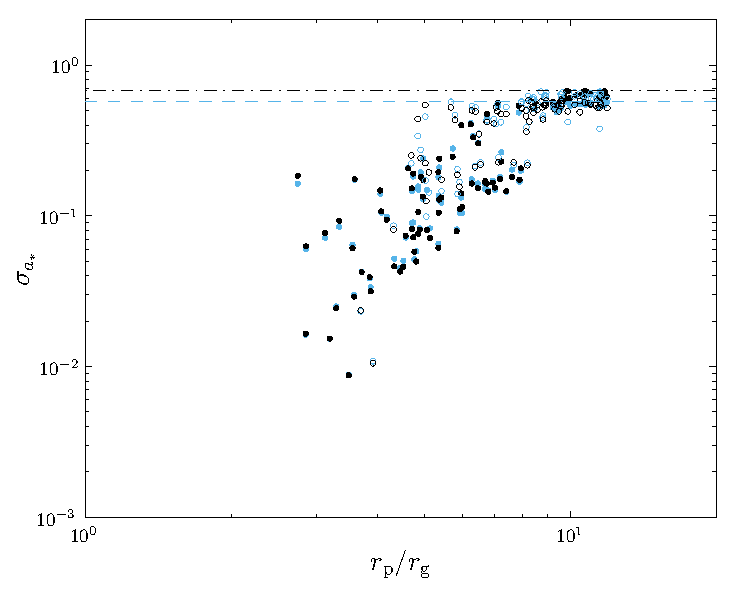
\includegraphics[width=0.475\textwidth]{./images/Fig_N4395_MCMC_sigmas_rp_2}} \\
\caption{Distribution widths as functions of periapsis $r\sub{p}$ for NGC 4395. Conventions are identical to those in \figref{sigmas-M32}.\label{fig:sigmas-N4395}}
\end{center}
\end{figure}

The widths, corresponding to potential parameter accuracies, improve rapidly with decreasing periapsis. The two widths, $\sigma\sub{SD}$ and $\sigma_{0.68}$, are typically of similar sizes, despite manifest non-Gaussianity. This is true for all parameters: the greatest differences are when the distributions are strongly multimodal. The fractional difference between the two widths may be up to $\sim 40\%$ for $\ln(M/M_\odot)$ and $a_\ast$; the widths for $\phi\sub{p}$ show the greatest difference, where $\sigma\sub{SD}$ may be a factor of a few larger than $\sigma_{0.68}$. Both $\sigma\sub{SD}$ and $\sigma_{0.68}$ tend to the appropriate limits for uninformative distributions.

In the best case, uncertainties in mass and spin may be only one part in $10^2$. As might be expected from \figref{detect}, M32 has the smallest widths followed by NGC 4945 and then NGC 4395. The spin width saturates about the value expected from a uniform distribution. At this point, we can no longer constrain the spin. The transition does not show any clear correlation with the magnitude of the spin, but is predominantly determined by the periapsis and SNR.

The other parameters show similar behaviour. The angular variables also reach maximum widths, corresponding to uninformative distributions. This does not appear to be directly tied to the spin width.

Potentially, an EMRB could place useful constraints on the mass and spin of an MBH if the periapse radius is small enough.\footnote{Here, we assume that a mass measurement is useful if its accuracy is smaller than the current measurement uncertainty, and a spin measurement is useful if it provides any constraint.} For M32 we require $r\sub{p} \lesssim 8 r\sub{g}$; for NGC 4945 we require $r\sub{p} \lesssim 8 r\sub{g}$ and $r\sub{p} \lesssim 7 r\sub{g}$ for mass and spin measurements, respectively, and for NGC 4395 we require $r\sub{p} \lesssim 9 r\sub{g}$ and $r\sub{p} \lesssim 8 r\sub{g}$, respectively. Since the range of useful periapses is small, we expect useful EMRBs originating from any individual galaxy to be rare. However, because there are many galaxies hosting potential sources, the probability of seeing any useful EMRBs need not be negligible. Therefore, EMRBs could be a useful astronomical tool.

\section{Summary and conclusions}\label{sec:extragal-End}

We have studied extreme-mass-ratio bursts from extragalactic sources. The SNR of EMRBs has a fundamental scaling with the system parameters. Removing these proportionalities gives a scaled SNR that can be specified as a function of the characteristic frequency $f_\ast$. Using these relations allows us to calculate the maximum distance to which EMRBs from a system containing an MBH of a given mass can be detected.

The MBH in our own Galaxy is by far the best source for bursts; however, it is also possible to detect bursts from extragalactic sources. In particular, M32 is a promising candidate. This is good news for any space-borne GW detectors, as EMRBs can be added to their list of potential sources.

Utilising the classic LISA design, EMRBs from a $10 M_\odot$ orbiting CO could be detected out to a distance of $\sim 100\units{Mpc}$. With the descoped eLISA design, this decreases to $\sim 10\units{Mpc}$. This may drastically reduce the chance of observing an EMRB. For both detectors, sensitivity is maximal for MBHs of $M \sim 10^6$--$10^7 M_\odot$, being at slightly higher masses for LISA than for eLISA. We can detect bursts from systems with high MBH spins out to greater distance; hence, the EMRB event rate would be enhanced if MBH spins naturally tend to higher values, perhaps as a consequence of accretion.

However, we must still be cautious: EMRBs may be rare and the event rate may prevent us from observing any over a realistic mission lifetime. Bursts from any given extragalactic source should be less common than from the Galactic Centre, although this may be slightly ameliorated by the larger number of galaxies hosting potential source systems. In the following chapter we shall construct a model to estimate the event rate for Galactic bursts. It is more difficult to perform a similar estimation for other galaxies as we do not have as detailed astrophysical measurement. However, we may use the Galactic event rate as a guide to predict the number of bursts per Milky Way equivalent galaxy.

Extragalactic EMRBs can provide good measurements of MBH mass and spin, but only across an extremely narrow range of periapses. We studied M32, NGC 4945 and NGC 4395 as examples. For all three we found that it is possible to extract information from bursts. The uncertainty may be one part in $10^2$--$10^3$ for M32, and slightly worse for NGC 4945 and NGC 4395, at about one part in $10^2$. These are not as good as the constraints from Galactic EMRBs, where the uncertainties could be as small as one part in $10^4$, but would still be of great astrophysical interest. These extragalactic MBHs are much harder to study than the MBH in our own Galaxy and we have not yet been able to measure a spin value even for that MBH. Any measurement of spin would give us a unique glimpse into the formation history of the host galaxy.

These results have been obtained assuming the classic LISA design. The first millihertz space-borne interferometer is likely to have a descoped design such as the proposed eLISA. This concept could be revised in the near future and so we have not used it to produce results. The effect of the reduced sensitivity would be to reduce the SNR and increase the widths of the posterior distributions. We expect the trends in \figref{sigmas-M32}, \ref{fig:sigmas-N4945} and \ref{fig:sigmas-N4395} to move upwards and saturate at smaller periapses.

Extreme-mass-ratio bursts could be used to place useful constraints on the mass and spin of a nearby MBH if the periapse radius is small enough. Considering the promising candidates of M32, NGC 4945 and NGC 4395, we find that $r\sub{p} \lesssim 8 r\sub{g}$ typically gives insightful constraints. Such orbits are likely to be rare, but just a single such burst from any of the potential galaxies could give us information that is otherwise inaccessible. This is a tantalising prospect.
